%! program = pdflatex

%\documentclass[12pt,a4paper]{memoir} % for a long document
\documentclass[10pt,letter,final,article,twocolumn]{article} % for a short document
\usepackage[left=0.25in,top=0.25in,right=0.25in,bottom=0.25in,nohead,nofoot]{geometry} 
\usepackage{titling,url}
\usepackage{graphicx}
% See the ``Memoir customise'' template for some common customisations
% Don't forget to read the Memoir manual: memman.pdf

\newcommand{\rpc}[1]{\emph{#1}}

\title{LWMR: Lightweight MapReduce}
\author{Athula Balachandran \\
{\tt abalacha@cs.cmu.edu}
\and
Wolfgang Richter \\
{\tt wolf@cs.cmu.edu}
\and
Erik Zawadzki \\
{\tt epz@cs.cmu.edu}}
\date{February 12, 2010} % delete this line to display the current date

%%% BEGIN DOCUMENT
\begin{document}

\pagestyle{empty}
\maketitle
\thispagestyle{empty}

\section{Problem Definition}

\section{Previous Work}

\section{Architecture}



\begin{figure}[htbp]
\begin{center}
\resizebox{0.9\columnwidth}{!}{
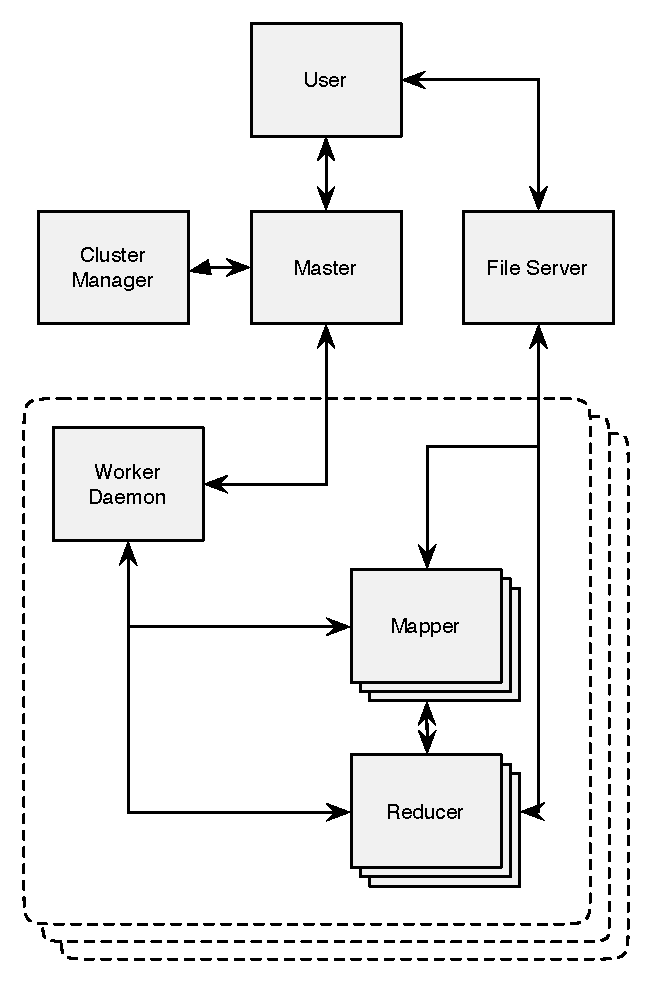
\includegraphics{Architecture.pdf}
}
\caption{A diagram of the major components of our architecture.}
\label{fig:arch}
\end{center}
\end{figure}


Our proposed architecture is shown in Figure~\ref{fig:arch}. This design is largely the same as the one presented in 
%\citet{dean04mapreduce}
?, with some additional detail. We will explain the architecture by taking the reader through a typical MapReduce job.

The user contacts a master process and submits the MapReduce job using the \rpc{SubmitJob} RPC call. The master job then requests, by RPC, that the worker daemon on each node starts one or more mappers. The master will try to place mapper jobs on nodes that have a replicated copy of the appropriate input split.

We are assuming in this phase of the work that the user has access to the complete cluster and that the current MapReduce job is the only job running on the system. Later iterations of our work will have to include interactions with a cluster resource manager.

 The worker daemon, upon receipt of a work request, spawns a new mapper thread for each request it gets. Because the worker daemon delays or rejects work requests the master is completely responsible for work scheduling.

The mapper thread buffers and writes the intermediate key-value pairs to local disk. Upon competition of the job, the mapper informs the worker daemon, and dies. The worker daemon then contacts the master to inform it that it has some complete work.

The master then 


\section{Milestone Deliverables}

\bibliographystyle{plain}
\bibliography{references}


\end{document}
